\documentclass[a4paper, 11pt]{article}
\usepackage{graphicx}
\usepackage{pdflscape}
\usepackage{titlesec}

\setcounter{secnumdepth}{4}

\usepackage[left=2cm, text={17cm, 24cm}, top= 3cm]{geometry}
\usepackage[utf8]{inputenc}
\usepackage[czech]{babel}

\begin{document}
 
    \begin{titlepage}
        
        \begin{center}
        
            {\Huge\textsc{ Vysoké učení technické v Brně\\
            \huge Fakulta informačních technologií}\\}
            
             \vspace{\stretch{0.382}}
             
             {\LARGE \Huge{IMP - Mikroprocesorové a vestavěné systémy\\ }}
             
                \vspace{0.5cm}
                
             {\LARGE ARM@FITkit3: Hodiny s budíkem na bázi modulu Real~Time~Clock~(RTC)}
               \vspace{\stretch{0.618}}
            
           \end{center} 
            
            {\LARGE Petr Kaška (xkaska01) \hfill \today}

    \end{titlepage}


    \section{Úvod}
    Tato dokumentace popisuje Real-Time Clock (RTC) budík a související klíčové principy, metody a protokoly týkající se jeho použití v daném systému nebo zařízení.

    \section*{Platforma}
    RTC budík je implementován na FITkit3.

    \section*{Konfigurační a Stavové Registry}
    RTC je nakonfigurován a sledován pomocí následujících konfiguračních a stavových registrů:

    \begin{itemize}
        \item RTC\_CR (RTC Control Register) -  Registry RTC\_CR jsou použity k ovládání RTC modulu. Nastavení obsahuje SWR (Software Reset) bit pro resetování RTC, OSCE (Oscillator Enable) pro povolení oscilátoru, a TCE (Time Counter Enable) pro zapnutí/ vypnutí RTC.
        \item RTC\_TCR (RTC Time Compensation Register) - Registrový obsah RTC\_TCR ovlivňuje kompenzaci času.
        \item RTC\_TSR (RTC Time Seconds Register) - Registrový obsah RTC\_TSR obsahuje aktuální sekundy RTC.
        \item RTC\_TAR (RTC Time Alarm Register) - Registrový obsah RTC\_TAR určuje čas pro alarm.
        \item UART5 C2 - Vynuluje bity pro vysílání a přijímání.
        \item UART5 BDH a UART5 BDL - Nastavují rychlost přenosu (baud rate) a nastavení stop bitů
        \item UART5 C4 a UART5 C1 - Nastavují různé parametry komunikace, jako jsou délka datových bitů a parita.
        \item UART5 MA1 a UART5 MA2 - Nastavují adresy pro režim match address (v tomto případě jsou deaktivovány).
        \item UART5 S2 - Nastavuje bity pro přerušení.
        \item UART5 C2 - Zapíná vysílač a přijímač.
        \item  A další registry dohledatelné v implementaci.
    \end{itemize}

    \section{Použití RTC budíku}
    RTC budík podporuje následující funkcionality a může být použit pro následující účely:
        \begin{itemize}
            \item Nastavení času pro hodiny. 
            \item Tři typy budících melodií.
            \item Tři typy svěletných show při buzení.
            \item Nastavení požadované budící konfigurace uživatelem.
            \item Nastavení budících cyklů.
            \item Nastavení času mezi jednotlivými budícími cykly. 
            \item Terminálové okno s barvami pro lepší orientaci uživatele v rozhraní.
            
        \end{itemize}

    \section{Návod}
    Pro spuštění budíka na zařízení FitKit3 jsou potřebné následující softwarové produkty: \textit{Windows 11}, \textit{Kinetis Design Studio}, \textit{PuTTY}

    \subsection{Nastavení}
    Připojte zařízení k počítačí a nahrajte zdrojový kód, následně spusťtě aplikaci \textit{PuTTY} na příslušném portu a s rychlostí \textit{115200}. 

    Po spuštění terminálového okna začne komunikace s aplikací. Jako první aplikace vyzve uživatele k inicializaci času. Po úspěšné inicializaci času přejdete do nastavení \textit{Přizpůsobení}. Nejprve výběr zvukové signalizace, při které si může uživatel poslechnout dostupné možnosti \textit{TRY1}, \textit{TRY2} nebo \textit{TRY3} a následně vybrat jednu z těchto možností \textit{FINAL1}, \textit{FINAL2} nebo \textit{FINAL3}. Po úspěšném výběru zvukové signalizace přijde na řadu výběr světelné signalizace, ve které si může nejprve prohlédnout dostupné světelné signalizace \textit{TRY1}, \textit{TRY2} a \textit{TRY3} a následně vybrat jednu z možností příslušným příkazem \textit{FINAL1}, \textit{FINAL2} a \textit{FINAL3}. Výbráním světelné signalizace se aplikace přepne do výběru \textit{počtu opakování}, ve kterém uživatel zadává číselnou hodnotu od 0 do 5. Při výběru 0 se aplikace přepne přímo do režimu \textit{nastavení času budíku}, jinak se přepne do režimu \textit{nastavení zpoždění}, ve kterém se vybírá doba mezi jednotlivými budícími cykly a následně se přepne do \textit{nastavení času budíku}. V tomto stavu si uživatel nastavuje čas spuštění aplikace. Po úspěšném nastavení se budík přepne do stavu \textit{aktivního čekání} a v příslušný čas se spustí. V tomto stavu lze zadat ještě následující příkazy.

    Čas je psán ve formátu \textit{YYYY-MM-DD\_HH:MM:SS} 

    \begin{itemize}
        \item \textit{OFF} - kompletně vypne budík.
        \item \textit{REBOOT} - kompletně restartuje celé hodiny.
        \item \textit{DISABLE} - vypne alarm.
        \item \textit{NEW\_ALL} - přepne do modu, znovunastavení budíku. Uživatel si může od začátku navolit přislušné přizpůsobení.
        \item \textit{NEW} - přepne do modu, znovunastavení budíku. Uživatel pouze nastavuje nový čas buzení s již nastaveným přizpůsobením
        \item \textit{HELP} - vypíše uživateli nápovědu.
        
    \end{itemize}

    \section{Implementace}

Při implementaci projektu bylo vycházeno ze schématu FITkit3 \cite{MAN}, manuálových stránek mikrokontroléru \cite{SCH}, a také jsme čerpali inspiraci z příkladů ze cvičení. Samotná implementace je rozdělena do několika zdrojových souborů a hlavičkových souborů, což pomáhá udržet strukturovanost a přehlednost kódu.

Celý zdrojový kód je organizován do funkcí, které jsou logicky seskupeny podle úkolů, které vykonávají. Při spuštění hlavní funkce main dojde nejprve k inicializaci různých komponent projektu. Toto zahrnuje nastavení mikrokontroléru a dalších zařízení. Poté cyklus \textit{while} běží neustále a nemá explicitní ukončovací podmínku.

Samotný cyklus je implementován jako konečný automat, což je způsob, jakým řídíme celý budík. Tímto automatem se nastavují globální proměnné, které jsou sdíleny mezi různými funkcemi a moduly. Tím se eliminuje potřeba složitě předávat parametry mezi funkcemi, což značně zjednodušuje strukturu kódu.

    Konkrétně to jsou zdrojové soubory a k nim příslusné hlavičkové soubory:

    \begin{itemize}
        \item date.c - funkce na zpracování času
        \item init.c - inicializace MCU, portů, UARTU a RTC.
        \item main.c - hlavní tělo programu.
        \item print.c - pomocné výpisové funkce
        \item state\_machine.c - konečný automat, který řídí činnost budíku
        \item str.c - čtení a zápis na terminál
        \item utilities.c - funkce na aktivní čekání výběr světel/zvuku a interupt handle 
    \end{itemize}

    \section{RTC modul}
        \subsection{Obsluha přerušení od RTC}
        Obsluha přerušení od RTC je zajištěna funkcí RTC\_IRQHandler. Tato funkce je vyvolána v okamžiku, kdy RTC modul generuje přerušení. V této funkcionalitě je implementována i část budíku. V případě, že má být aktivován budík, provede se přenastavení času pro odložené buzení.
    
    \subsection{Nastavení RTC modulu}
    RTC modul vyžaduje časové údaje ve formátu 32 bitového čísla v sekundách. Uživatel zadává čas ve formátu "YYYY-MM-DD\_HH:MM:SS," což je lidsky čitelný formát. Pro konverzi tohoto času do požadovaného 32bitového formátu slouží dvě funkce: time\_load a time\_convert.
    
    \subsection{input\_time}
    Tato funkce provádí konverzi času z formátu "YYYY-MM-DD HH:MM:SS" do počtu sekund od epochy (1.1.1970). Pro tuto konverzi využívá funkci strftime z knihovny time.h, která převede lidsky čitelný formát na počet sekund. Výsledek této konverze je počet sekund od 1.1.1970 do zadaného času uživatelem.
    
    \subsection{time\_to\_str}
    Tato funkce provádí opačný proces, tj. konverzi počtu sekund od epochy zpět na lidsky čitelný formát "YYYY-MM-DD HH:MM:SS". Tato funkce se používá zejména k informování uživatele o aktuálním čase v RTC.

   \newpage 
    \begin{figure}
        \section{Stavový automat}
        \centering
        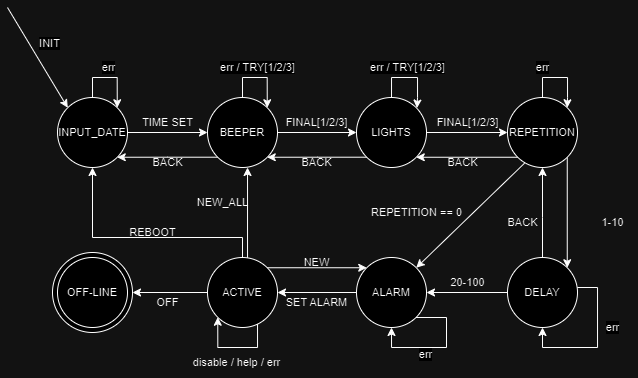
\includegraphics[width=\textwidth]{imp.drawio.png}
        \caption{\label{fig:The-caption}Konečný automat budíku}
    \end{figure}
\newpage

    \bibliographystyle{czechiso}
    \renewcommand{\refname}{Literatura}
	\bibliography{cite}
\end{document}
 
